% !TeX spellcheck = da_DK
\subsection{Spændingsforsyning}
Til systemet anvendes to 9V batterier som spændingsforsyning koblet i et splitsupply, hvilket er illustreres på \figref{fig:splitsupply}. Splitsupply medvirker til at sysemet opnår et arbejdsområde fra $\pm$ 9V. Systemet opsættes så den positive pol på det ene batteri tilkobles den negative pol på det andet batteri, på denne måde opnås en jordforbindelse. Den negative pol i batteri i det første batteri anvendes som systemets negative forsyningsspænding og indikeres med $-V_{cc}$, mens det andet batteri anvendes som den positive spændingsforsyning og indikeres med $+V_{cc}$.
Da batterierne ikke leverer den samme spænding over hele batteriernes levetid, skal batteriet skiftes ud når det ikke leverer den spænding som er nødvendig for systemet. Batteriernes levetid afhænger af hvor mange ampere systemet trækker ud. Da feedbacken kræver en spænding på xx V skal systemet minimum leverer en spænding på xx V. Derfor kræver systemt en minimal spænding på xx V.

\begin{figure}[H]
\centering
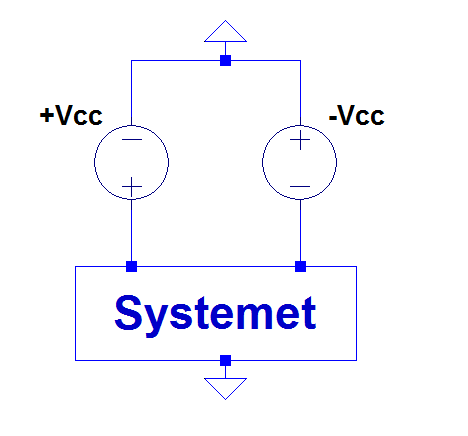
\includegraphics[scale=0.5]{figures/cProblemloesning/Splitsupply.PNG}
\caption{Figuren viser opsætningen af et splitsupply spændingsforsyning. Ved testning af batterierne vil $-V_{cc}$ og $+V_{cc}$ illustrerer henholdsvis den positive og negative pol på batterierne.}
\label{fig:splitsupply}
\end{figure}

\subsubsection{Test af spændingsforsyning}
Batteriernes levetid undersøges ved at teste hvor mange ampere systemet bruger. På baggrund af dette vil informationen omkring batteriernes levetid give en estimering af hvornår de skal udskiftes. Testningen foregår ved en serieforbindelse mellem den negative spændingsforsyning $-V_{cc}$ eller positive spændingsforsyning $+V_{cc}$ og systemet. Selve opsætningen af testen illustreres på \figref{spaendingsforsyning}.
